\documentclass[12pt]{scrartcl}%{article}
\usepackage{scrlayer-scrpage}
\pagestyle{scrheadings}
\usepackage{tabularx}
\usepackage{lastpage}
\usepackage{amsmath,amssymb}
\usepackage[yyyymmdd,hhmmss]{datetime}
\usepackage{graphicx}
\usepackage[siunitx, RPvoltages]{circuitikz}

\usepackage[english]{babel}
\usepackage[T1]{fontenc}
\usepackage{lmodern}
\usepackage{csvsimple}
\usepackage[ansinew]{inputenc}  % Unix
  % \usepackage[ansinew]{inputenc}  % Windows
  % \usepackage[applemac]{inputenc} % Mac
  
\usepackage[a4paper, left=2cm, right=2cm, top=3.0cm, bottom = 2.5cm]{geometry}
\setlength{\headsep}{0.5cm}

\ihead{\includegraphics[scale=0.18]{Zahner_Logo.pdf}}

\usepackage{lmodern}
\cfoot{Page \thepage}

\usepackage[thmmarks,amsmath,hyperref,noconfig]{ntheorem}
  
\usepackage[colorlinks,
pdfpagelabels,
pdfstartview = FitH,
bookmarksopen = true,
bookmarksnumbered = true,
linkcolor = black,
plainpages = false,
hypertexnames = false,
citecolor = black] {hyperref}  


\usepackage{color}
\definecolor{white}{rgb}{1,1,1}
\definecolor{darkred}{rgb}{0.3,0,0}
\definecolor{darkgreen}{rgb}{0,0.3,0}
\definecolor{darkblue}{rgb}{0,0,0.3}
\definecolor{pink}{rgb}{0.78,0.09,0.51}
\definecolor{purple}{rgb}{0.28,0.24,0.55}
\definecolor{orange}{rgb}{1,0.6,0.0}
\definecolor{grey}{rgb}{0.4,0.4,0.4}


\DeclareMathOperator{\GL}{GL}
\newcommand{\N}{\mathbb{N}}
\newcommand{\Z}{\mathbb{Z}}
\newcommand{\Q}{\mathbb{Q}}
\newcommand{\R}{\mathbb{R}}
\newcommand{\C}{\mathbb{C}}
\newcommand{\cP}{{\mathcal P}} 

\begin{document}
\vspace*{30mm}
\begin{center}
  \title{Capacitor Test Report}
  \textbf{{\huge Capacitor Test Report}}
\end{center}
\vspace*{40mm}


\section{Informations}
\vspace{5mm}
\begin{center}
  \begin{tabularx}{0.8\textwidth}{| X | X |}
    \hline
                               &                    \\
    \textbf{Test object name}: & C1234 \\
                               &                    \\
    \hline
                               &                    \\
    \textbf{Date of test}:     & \today             \\
                               &                    \\
    \hline
                               &                    \\
    \textbf{Time of test}:     & \currenttime       \\
                               &                    \\
    \hline
  \end{tabularx}
\end{center}
\newpage

\section{Measurement}

\subsection{CV}
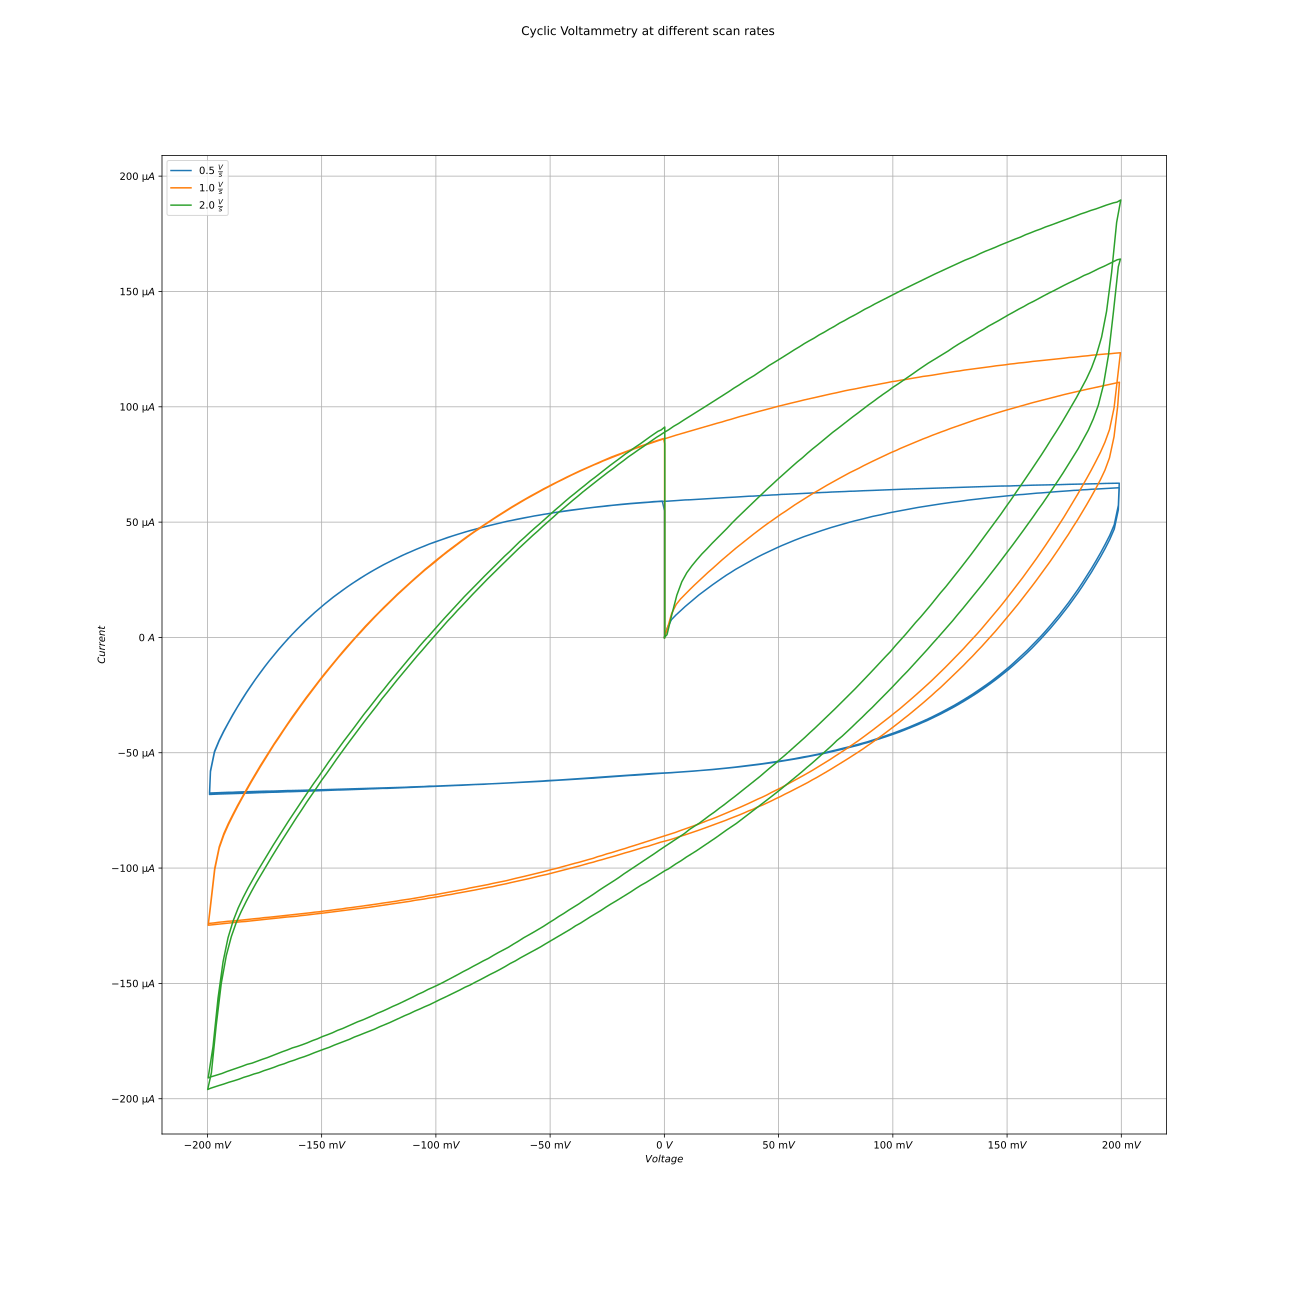
\includegraphics[width=1\textwidth]{ CV.pdf }

\newpage

\subsection{EIS}
\includegraphics[width=1\textwidth]{ EIS.pdf }

\begin{center}
  \begin{tabular}{c|c|c}
    \bfseries Frequency $[Hz]$ & \bfseries |Impedance| $[\Omega]$ & \bfseries Phase [\textdegree]
    \csvreader[head to column names, /csv/separator=semicolon]{ EIS.csv }{}
    {                                                                                             \\\hline \Frequency & \Impedance & \Phase}
  \end{tabular}
\end{center}

\section{Evaluation}

\subsection{CV}

The basic equation for the relationship between voltage, capacitance and charge is:

\begin{center}
  \begin{math}
    C = \dfrac{Q}{U}
  \end{math}
  or
  \begin{math}
    C = \dfrac{I * t}{U}
  \end{math}
\end{center}
\noindent
Where C = capacity, Q = charge, I = current, t = time and U = voltage. If we assume a linearly increasing or decreasing voltage (dU/dt - as in CV) as well as a voltage of zero volts at the beginning of the experiment, we get the following equation:

\begin{center}
  \begin{math}
    C = \dfrac{I}{\frac{dU}{dt}} = \dfrac{\dfrac{592.838\mu A - (-591.877\mu A)}{2}}{0.25 \frac{V}{s}} = 2.369mF
  \end{math}
\end{center}

\subsection{EIS}

The parameters of the following simplified equivalent circuit model of a capacitor are fitted with the impedance spectrum:

\begin{center}
  \begin{circuitikz}[european]
    \draw (0,0)
    to[R = $R_0$] (2,0)
    to[C = $C_0$] (4,0)
    to[L = $L_0$] (6,0)
    ;
  \end{circuitikz}
\end{center}

\noindent
Results of fitting the model parameters to the measured data are shown in the table:
\begin{center}
  \begin{tabular}{|c|c|c|}
    \hline
    \textbf{Element} & \textbf{Fitted Value}   & \textbf{Fit Error}              \\
    \hline
    $R_0$            & 51.749m$\Omega$  & 5.3\%  \\
    \hline
    $C_0$            & 2.130mF & 4.8\% \\
    \hline
    $L_0$            & 11.493nH  & 40.2\%  \\
    \hline
  \end{tabular}
\end{center}

\vspace{5mm}
\noindent
In the following figure, the measurement data and the curve for the simulated model with the fitted parameters are shown:
\begin{center}
  \includegraphics[width=1\textwidth]{ EIS_fitted.pdf }
\end{center}

\end{document}